\subsection{Numerical Evaluation}\label{sec:application:lte_video:numerical_evaluation}

In this section we study the metrics introduced in \refsec{sec:application:lte_video:system_model:model_assumptions:metrics} on the different transmission mechanisms.

First, we study the impact of the considered transmission mechanisms on the energy consumption and the wasted traffic. 
Then, in \refsec{sec:application:lte_video:connection_count} we consider the impact of the connection count for the \streaming mechanisms and varying values of the parameters \emph{stop threshold} \bufferlower and \emph{threshold size} \buffersize in more detail.

We consider a video of \(\videolength=\SI{1600}{\second}\) length which is viewed on a \gls{UE} with \gls{LTE} access.
The median of available downlink throughput in current \gls{LTE} networks is \(\bandwidth = \SI{12.74}{\mega\bit\per\second}\) \cite{Huang2012}.
A wide set of video bitrates between \SIlist{1;50}{\mega\bit\per\second} is in use~\cite{YouTube2013}.
In order to prevent stalling, we consider bitrates between \SIrange{1}{10}{\mega\bit\per\second}, staying below the available network bandwidth.
For the \streaming mechanism, a stop threshold of \(\bufferlower = \SI{4}{\second}\) and a threshold size of \(\buffersize = \SI{32}{\second}\) were selected.
Furthermore, we specify a prebuffering duration of \(\streamingstart = \SI{5}{\second}\).

We conduct our study using deterministic discrete event simulation which uses no random variables.
The wasted traffic is obtained analytically using the abort behaviour model.
Thus, all results are exact under the previously stated assumptions.

\subsubsection*{Energy Consumption}\label{sec:application:lte_video:numerical_evaluation:energy_consumption}
First, we study the influence of both video bitrate as well as the selected download mechanism on energy consumption in \reffig{fig:application:lte_video:numerical_evaluation:energy_consumption:bitrate2energy}.
\begin{figure}
  \centering
  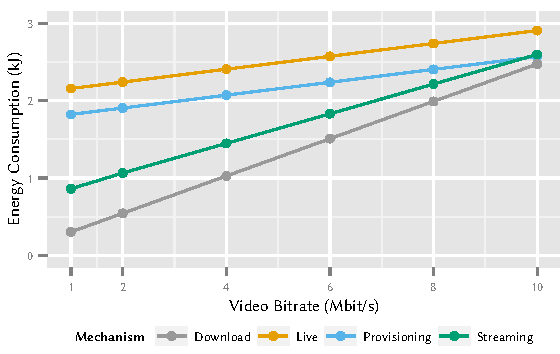
\includegraphics{application/lte_video/numerical_evaluation/figures/bitrate2energy}
  \caption{Influence of bitrate and download mechanism on energy consumption}
  \label{fig:application:lte_video:numerical_evaluation:energy_consumption:bitrate2energy}
\end{figure}

We consider the \download mechanism and observe that it consumes the least amount of energy.
Here the video is downloaded with full bandwidth, as seen in \reffig{fig:application:lte_video:system_model:video_model}, resulting in a very short energy intensive download phase and a longer energy un-intensive playback phase.
For the \live mechanism we observe the opposite, i.e. the highest energy consumption for all bandwidths.
If this mechanism is used, the used bandwidth equals the video bitrate.
Thus, the download requires the same amount of time as the playback, resulting in the highest possible energy consumption.
The \serviceprovisioning method uses a higher bandwidth, thus reducing the overall download time.
This reduced download time decreases the energy consumption when compared to the \live mechanism, even though the bandwidth used for downloading is increased to \SI{120}{\percent}.
For the \streaming mechanism we observe an energy consumption slightly higher than the \download mechanism.
As the bitrate of the video increases, the energy consumption increases as well.
This is due to the fact that a higher video bitrates require larger downloads.
For video bitrates approaching the available bandwidth the \streaming mechanism degenerates to the \live mechanism, as no prebuffering is possible.
We conclude that the \download and \streaming mechanisms outperform \live and \serviceprovisioning with regard to energy consumption.

\subsubsection*{Wasted Traffic}\label{sec:application:lte_video:numerical_evaluation:wasted_traffic}
Next, we consider the wasted traffic as a metric of the transmission mechanism quality.
If a user completely watches a video, no traffic is wasted.
Thus, we consider only the cases where a user stops the playback before the video is finished.
\begin{figure}
  \centering
  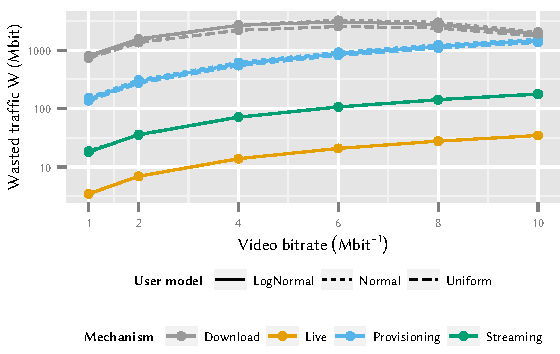
\includegraphics{application/lte_video/numerical_evaluation/figures/bitrate2lostData}
  \caption{Influence of bitrate, download mechanism and user model on wasted traffic}
  \label{fig:application:lte_video:numerical_evaluation:energy_consumption:bitrate2lostData}
\end{figure}
In \reffig{fig:application:lte_video:numerical_evaluation:energy_consumption:bitrate2lostData} we study the wasted traffic for different video bitrates.
We consider the different transmission mechanisms introduced in \refsec{fig:application:lte_video:system_model:video_model} as well as the previously introduced user models.
We observe that the choice of user model has no significant impact on the wasted traffic.
For the \download mechanism, the amount of wasted traffic increases up to a video bitrate of \SI{6}{\mega\bit\per\second}, then the wasted traffic decreases as only video data which has been prebuffered can be lost if the user aborts the video.
As we assume a available bandwidth of \SI{12.74}{\mega\bit\per\second}, the bandwidth available for prebuffering decreases as the bitrate increases, resulting in lower amounts of wasted traffic for high video bitrates.
For the \live mechanism, we see that the wasted traffic for all user models is very low, but wasted traffic exists.
This is due to the traffic already sent by the server while the \gls{UE} is still waiting for promotion from \rrcidle to \rrcconnected, i.e. a short prebuffering phase exists.
As the bandwidth increases with the video bitrate, the wasted traffic increases as well.
Next, we consider the \serviceprovisioning approach and see an increase of wasted traffic as the video bitrate increases, due to the fact that the bandwidth used for continuous download is a factor of the video bitrate.
A higher video bitrate results in the download of the video being completed earlier, which leads to more wasted traffic.
Similar results can be seen for the \streaming mechanism, which results in more wasted traffic than the \live mechanism, but significantly less traffic than the \serviceprovisioning mechanism.
This is due to the fact that if the user aborts, at least the amount of video given by the \emph{stop threshold} \bufferlower and at most the complete buffer, given by the \emph{stop threshold} and the \emph{threshold size} are lost.
We have observed that the choice of user model results in no qualitative changes in wasted traffic.
As we have seen, the \download and \streaming mechanisms provide best results with regard to energy consumption.
However with regard to wasted traffic, the \live and \streaming mechanisms are most suited.
Thus, the \streaming mechanism seems to be a good compromise.
The network operator can select a tradeoff between energy consumption and wasted traffic as discussed in the next section.
From now on, we only consider the uniformly distributed user model.

\subsubsection*{Connection Count}\label{sec:application:lte_video:connection_count}
The \gls{ISP} is interested in reducing the number of connections occurring during video transmission.
Thus, we quantify the impact of the selected video transmission mechanism on the connection count, which directly correlates with the occurring signalling.
\begin{figure}
  \centering
  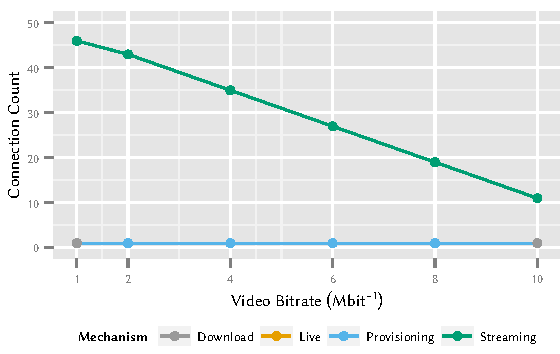
\includegraphics{application/lte_video/numerical_evaluation/figures/bitrate2connections}
  \caption{Influence of bitrate and download mechanism on connection counts}
  \label{fig:application:lte_video:numerical_evaluation:energy_consumption:bitrate2connections}
\end{figure}

In \reffig{fig:application:lte_video:numerical_evaluation:energy_consumption:bitrate2connections} we study the impact of the different transmission mechanisms on the number of connections per transmission and thus the amount of generated signalling.
We observe that for the transmission mechanisms download, live, provisioning the number of connections is constantly one, independent of the selected bitrate \bitrate.
This is due to the fact that in these transmission mechanisms the video is transmitted in one chunk.
For streaming, the number of connections decreases as the video bitrate increases.
Here, a connection occurs each time the buffer is refilled.
For larger bitrates, refilling the buffer requires a longer transmission.
As the maximum time of video transmission is upper bounded by the video length, longer buffering phases result in a smaller total amount of buffering phases and thus in less connections per video transmission.

\begin{figure}
  \centering
  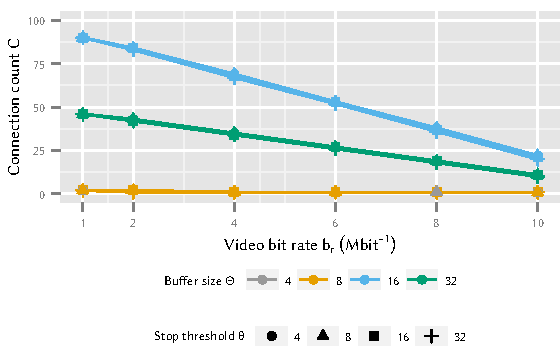
\includegraphics{application/lte_video/numerical_evaluation/figures/bitrate2connections_parameters}
  \caption{Influence of bitrate and selected parameters on connection counts for the streaming mechanism}
  \label{fig:application:lte_video:numerical_evaluation:energy_consumption:bitrate2connections_parameters}
\end{figure}

Next, we consider the impact of the lower buffer threshold \bufferlower and buffer size \buffersize on the number of connections \connectioncount caused by the \streaming mechanism.
In \reffig{fig:application:lte_video:numerical_evaluation:energy_consumption:bitrate2connections_parameters} we observe that while the buffer size has a significant impact on the number of connections during a video transmission, the lower buffer threshold has almost no impact.
For buffer sizes of \SIrange{4}{8}{\second}, no signalling occurs.
This is due to the fact that, as discussed in \refsec{sec:application:lte_video:system_model:lte_network_model}, the connection timeout in \gls{UE} is configured as \SI{11.576}{\second}.
Thus, for this low buffer sizes the \gls{UE} does not disconnect from the network.
Furthermore, we observe that as the buffer size increases, the number of connections decreases.
Refilling larger buffers requires, similar to larger bitrates, longer transmission times.
Thus, due to the total upper bound on the transmission time, less download phases can occur during the transmission.